\documentclass[12pt,a4paper]{article}

\usepackage{graphicx}% Include figure files
\usepackage{dcolumn}% Align table columns on decimal point
\usepackage{bm}% bold math
%\usepackage{hyperref}% add hypertext capabilities
%\usepackage[mathlines]{lineno}% Enable numbering of text and display math
%\linenumbers\relax % Commence numbering lines

%\usepackage[showframe,%Uncomment any one of the following lines to test 
%%scale=0.7, marginratio={1:1, 2:3}, ignoreall,% default settings
%%text={7in,10in},centering,
%%margin=1.5in,
%%total={6.5in,8.75in}, top=1.2in, left=0.9in, includefoot,
%%height=10in,a5paper,hmargin={3cm,0.8in},
%]{geometry}

\usepackage{multicol}%Para hacer varias columnas
\usepackage{multicol,caption}
\usepackage{multirow}
\usepackage{cancel}

\setlength{\topmargin}{-1.0in}
\setlength{\oddsidemargin}{-0.3pc}
\setlength{\evensidemargin}{-0.3pc}
\setlength{\textwidth}{6.75in}
\setlength{\textheight}{9.5in}
\setlength{\parskip}{0.5pc}

\usepackage[utf8]{inputenc}
\usepackage{expl3,xparse,xcoffins,titling,kantlipsum}
\usepackage{graphicx}
\usepackage{xcolor} 
\usepackage{nopageno}
\usepackage{lettrine}
\usepackage{caption}
\captionsetup[table]{name=Tabla}
\renewcommand{\figurename}{Figura}
\usepackage{float}
\renewcommand\refname{Bibliograf\'ia}
\usepackage{amssymb}
\usepackage{amsmath}
\usepackage[rightcaption]{sidecap}
\usepackage[spanish]{babel}

% CABECERA Y PIE DE PÁGINA %%%%%
\usepackage{fancyhdr}
\pagestyle{fancy}
\fancyhf{}

\begin{document}
\noindent 1. En una distribución tipo Maxwell la fracción de partículas moviéndose con velocidad $v$ y $v+dv$ es
\begin{equation}
    \frac{dN}{N} = 4 \pi ( \frac{m}{2\pi kT})^ \frac{3}{2}  exp(-\frac{m v^2}{2kT}) v^2 dv
\end{equation}
donde N es el número total de partículas.
El promedio o valor esperado de $v^n$ se define como $< v^n > = N ^{-1} \int v^n dN$
Demuestre  que :
\begin{equation*}
    < v^n > = ( \frac{2kT}{m} )^{\frac{n}{2}} \frac{(\frac{n+1}{2})!}{(\frac{1}{2})!}
\end{equation*}

de la ec. (1)
\begin{equation*}
    N^{-1} = \frac{4 \pi ( \frac{m}{2\pi kT})^ \frac{3}{2}  exp(-\frac{m v^2}{2kT}) v^2 dv}{dN}
\end{equation*}
así, sustituyendo 
\begin{equation*}
    < v^n > = \frac{4 \pi ( \frac{m}{2\pi kT})^ \frac{3}{2}  exp(-\frac{m v^2}{2kT}) v^2 dv}{dN} \int v^n dN
\end{equation*}
si reordenamos y tratamos diferenciales como fracciones xd

\begin{equation*}
    < v^n > = 4 \pi ( \frac{m}{2\pi kT})^ \frac{3}{2}  \int exp(-\frac{m v^2}{2kT}) v^{n + 2} dv 
\end{equation*}
ahora usemos cambio de variable para resolver esa integral

Sea $u^2 = \frac{m v^2}{2kT}$ y $\cancel{2}udu = \cancel{2}\frac{mv}{2kT} dv$ , $du = \frac{m}{2kT} dv$, entonces

\begin{equation*}
     <v^n > = 4 \pi (\frac{m}{2 \pi k T})^{\frac{3}{2}} (\frac{m}{2kT}) ^{-(n+1)}\int  e^{-u^2} u^{n+2} du
\end{equation*}

\begin{equation*}
    = 4 \pi (\frac{m}{2 \pi k T})^{\frac{3}{2}} ((\frac{m}{2kT}) ^{-(n+1)})^{\frac{2}{2}}\int  e^{-u^2} u^{n+2} du = 4 \pi (\frac{m}{2 \pi k T})^{\frac{3}{2}} (\frac{m}{2kT}) ^{-(n+3)/2}\int  e^{-u^2} u^{n+2} du 
\end{equation*}

haciendo otro cambio de variable, $x = u^2$, $dx = 2 u du$ 

\begin{equation*}
    < v^n > = 4 \pi (\frac{m}{2 \pi k T})^{\frac{3}{2}} (\frac{m}{2kT}) ^{-(n+3)/2}\int  e^{-u^2} u^{n+2} du = 4 \pi (\frac{m}{2 \pi k T})^{\frac{3}{2}} (\frac{m}{2kT}) ^{-(n+3)/2} \frac{1}{2} \int e^{-x} x^{(n+1)/2} dx 
\end{equation*}

\begin{equation*}
    = 4 \pi (\frac{m}{2 \pi k T})^{\frac{3}{2}} (\frac{m}{2kT}) ^{-(n+3)/2} \frac{1}{2} \Gamma(\frac{n+3}{2})
\end{equation*}

\begin{equation*}
    = 2 \pi (\frac{2kT}{m})^{\frac{n}{2}} \Gamma (\frac{n+3}{2})
\end{equation*}











\newpage
\noindent 2. Se muestra en la figura (1) parte de una cicloide cuyas ecuaciones parametrícas son:
\begin{equation*}
    x = a(\theta + sen\theta)
\end{equation*}
\begin{equation*}
    y = a(1 - cos \theta    )
\end{equation*}

\noindent Demuestre que el tiempo que tarda una partícula para desliarse sin fricción a lo largo de la curva desde el punto $(x_1, y_1)$ hasta el origen, está dado por

\begin{equation*}
    t = \sqrt{\frac{a}{g}} \int \limits_{0}^{y_1} \frac{dy}{\sqrt{y(y_1 - y)}}
\end{equation*}

\begin{figure}[h!]
    \centering
    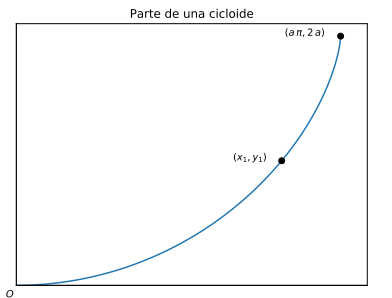
\includegraphics{Ejercicios_Tema_01_Semana_03.pdf - Google Chrome 22_03_2021 01_34_00 p. m. (2).png}
    \caption{}
\end{figure}
\noindent Sugerencia: Duemuetra que la longitud del elemento de arco es
\begin{equation*}
    ds = \sqrt{\frac{2a}{y}} dy
\end{equation*}
Evalúa la integral para demostrar que el tiempo es independiente de la posición inicial $y_1$

\begin{equation*}
    \frac{ds}{dt} ^2 = \frac{d x}{d \theta} ^2 + \frac{d y}{ d \theta} ^2 = (a + a \cos{\theta})^2 + (a \sen{\theta})^2
\end{equation*}

\begin{equation*}
    = a^2 + 2a^2 \cos{\theta} + a^2 \cos^2{\theta} + a^2 \sen^2{\theta} = a^2 (1+ 2 \cos{\theta} + (\cancel{\cos^2{\theta} + \sen^2{\theta}})) 
\end{equation*}

\begin{equation*}
    = a^2 (2 + 2 \cos{\theta})  = 2 a^2 (1 + \cos{\theta})
\end{equation*}

\begin{equation*}
    ds = \sqrt{ 2 a^2(1 + \cos{\theta})} = \sqrt{\frac{2 a^2 (1+ \cos{\theta})( 1 - \cos{\theta})}{1- \cos{\theta}}}= \sqrt{\frac{2 a^2 (1 - \cos^2{\theta})}{1- \cos{\theta}}} = \sqrt{\frac{2 a^3 \sen^2{ \theta}}{a (1- \cos{\theta})}} 
\end{equation*}

\begin{equation*}
    = \sqrt{\frac{2a}{a (1- \cos{\theta})}} a \sen{\theta} = \sqrt{\frac{2a}{y}} dy
\end{equation*}

\begin{equation*}
    \cancel{m}g(y_1-y) = \frac{1}{2} \cancel{m} v^2 - \cancel{\frac{1}{2} m v_0 ^2} 
\end{equation*}

\begin{equation*}
    v = \sqrt{2g (y_1 - y)} = \frac{ds}{dt}
\end{equation*}

\begin{equation*}
     dt = \frac{ds}{\sqrt{2g(y_1 - y)}} = \frac{\sqrt{\frac{2a}{y}} dy}{\sqrt{2g(y_1 - y)}}= \sqrt{\frac{\cancel{2}a}{\cancel{2} g y (y_1 - y)}} dy
\end{equation*}

\begin{equation*}
    = \sqrt{\frac{a}{y}} \frac{dy}{\sqrt{y (y_1 - y)}}
\end{equation*}

\begin{equation*}
    \int dt = \int \limits_{0}^{y_1} \sqrt{\frac{a}{g}} \frac{dy}{\sqrt{y (y_1 - y)}} = \sqrt{\frac{a}{g}} \int \limits_{0}^{y_1} \frac{dy}{\sqrt{y (y_1 - y)}}
\end{equation*}

\begin{equation*}
    t = \sqrt{\frac{a}{g}} \int \limits_{0}^{y_1} \frac{dy}{\sqrt{y (y_1 - y)}} = \sqrt{\frac{a}{g}} \int \limits_{0}^{y_1} \frac{a \sen{\theta} d\theta}{\sqrt{a(1-\cos{\theta}) (y_1 - a(1- \cos{\theta}))}}
\end{equation*}

\begin{equation*}
    = 
\end{equation*}






\end{document}
